\documentclass[conference]{IEEEtran}
\IEEEoverridecommandlockouts
% The preceding line is only needed to identify funding in the first footnote. If that is unneeded, please comment it out.
\usepackage[numbers]{natbib}
\usepackage{amsmath,amssymb,amsfonts}
\usepackage{algorithmic}
\usepackage{graphicx}
\usepackage{textcomp}
\usepackage{xcolor}
\usepackage{todonotes}
\def\BibTeX{{\rm B\kern-.05em{\sc i\kern-.025em b}\kern-.08em
    T\kern-.1667em\lower.7ex\hbox{E}\kern-.125emX}}

\setlength{\abovecaptionskip}{0pt plus 3pt minus 2pt}

\setlength{\abovedisplayskip}{2pt}
\setlength{\belowdisplayskip}{2pt}

\begin{document}

\title{Balanced Information Gathering and Goal-Oriented Actions in Shared Autonomy
\thanks{This work was supported by an NSF CRII Award \#1566612.}
}

\author{\IEEEauthorblockN{Connor Brooks}
\IEEEauthorblockA{\textit{Department of Computer Science} \\
\textit{University of Colorado Boulder}\\
Boulder, USA \\
connor.brooks@colorado.edu}
\and
\IEEEauthorblockN{Daniel Szafir}
\IEEEauthorblockA{\textit{Department of Computer Science \& ATLAS Institute} \\
\textit{University of Colorado Boulder}\\
Boulder, USA \\
daniel.szafir@colorado.edu}
}
\maketitle

\begin{abstract}
Robotic teleoperation can be a complex task due to factors such as high degree-of-freedom manipulators, operator inexperience, and limited operator situational awareness. To reduce teleoperation complexity, researchers have developed the shared autonomy control paradigm that involves joint control of a robot by a human user and an autonomous control system. We introduce the concept of active learning into shared autonomy by developing a method for systems to leverage \textit{information gathering}: minimizing the system's uncertainty about user goals by moving to information-rich states to observe user input. We create a framework for balancing information gathering actions, which help the system gain information about user goals, with goal-oriented actions, which move the robot towards the goal the system has inferred from the user. We conduct an evaluation within the context of users who are multitasking that compares pure teleoperation with two forms of shared autonomy: our balanced system and a traditional goal-oriented system. Our results show significant improvements for both shared autonomy systems over pure teleoperation in terms of belief convergence about the user's goal and task completion speed and reveal trade-offs across shared autonomy strategies that may inform future investigations in this space.
\end{abstract}

\begin{IEEEkeywords}
Shared autonomy; human-robot teaming; active learning; inverse reinforcement learning; assistive teleoperation
\end{IEEEkeywords}

\section{Introduction}

Shared autonomy is a robotic control paradigm that blends user input with an autonomous control system \cite{dragan2012formalizing, dragan2013policy, gopinath2017human}. This paradigm can be especially useful in cases where human users interact with high degree-of-freedom systems and are unable to provide sufficient control input due to inexperience with the system, user distractions, physical or cognitive limitations, or other factors. Shared autonomy enables robots to make use of both the information that is provided by a human user and the robot's own internal control and perception systems. For these two sources of control to work together effectively, it is critical that they share a common goal.

Previous work has suggested that one method of enhancing human-robot interaction is to improve robot understanding of natural and implicit cues from humans rather than only supporting explicit communication \cite{goodrich2003seven}. In shared autonomy, robots might similarly learn about user goals in an implicit manner by observing user control actions rather than requiring users to explicitly specify their goals. Implicitly learning user goals may support more fluid interaction and better support scenarios in which explicit goal designation is infeasible due to limitations in user controls, difficulties in describing the state space, or other factors. To learn user goals, shared autonomy systems build a belief model of possible goals by observing the user-provided control actions at different states. Intuitively, this involves abstracting the user's individual actions to see them as a part of a larger goal-oriented policy.

\begin{figure}
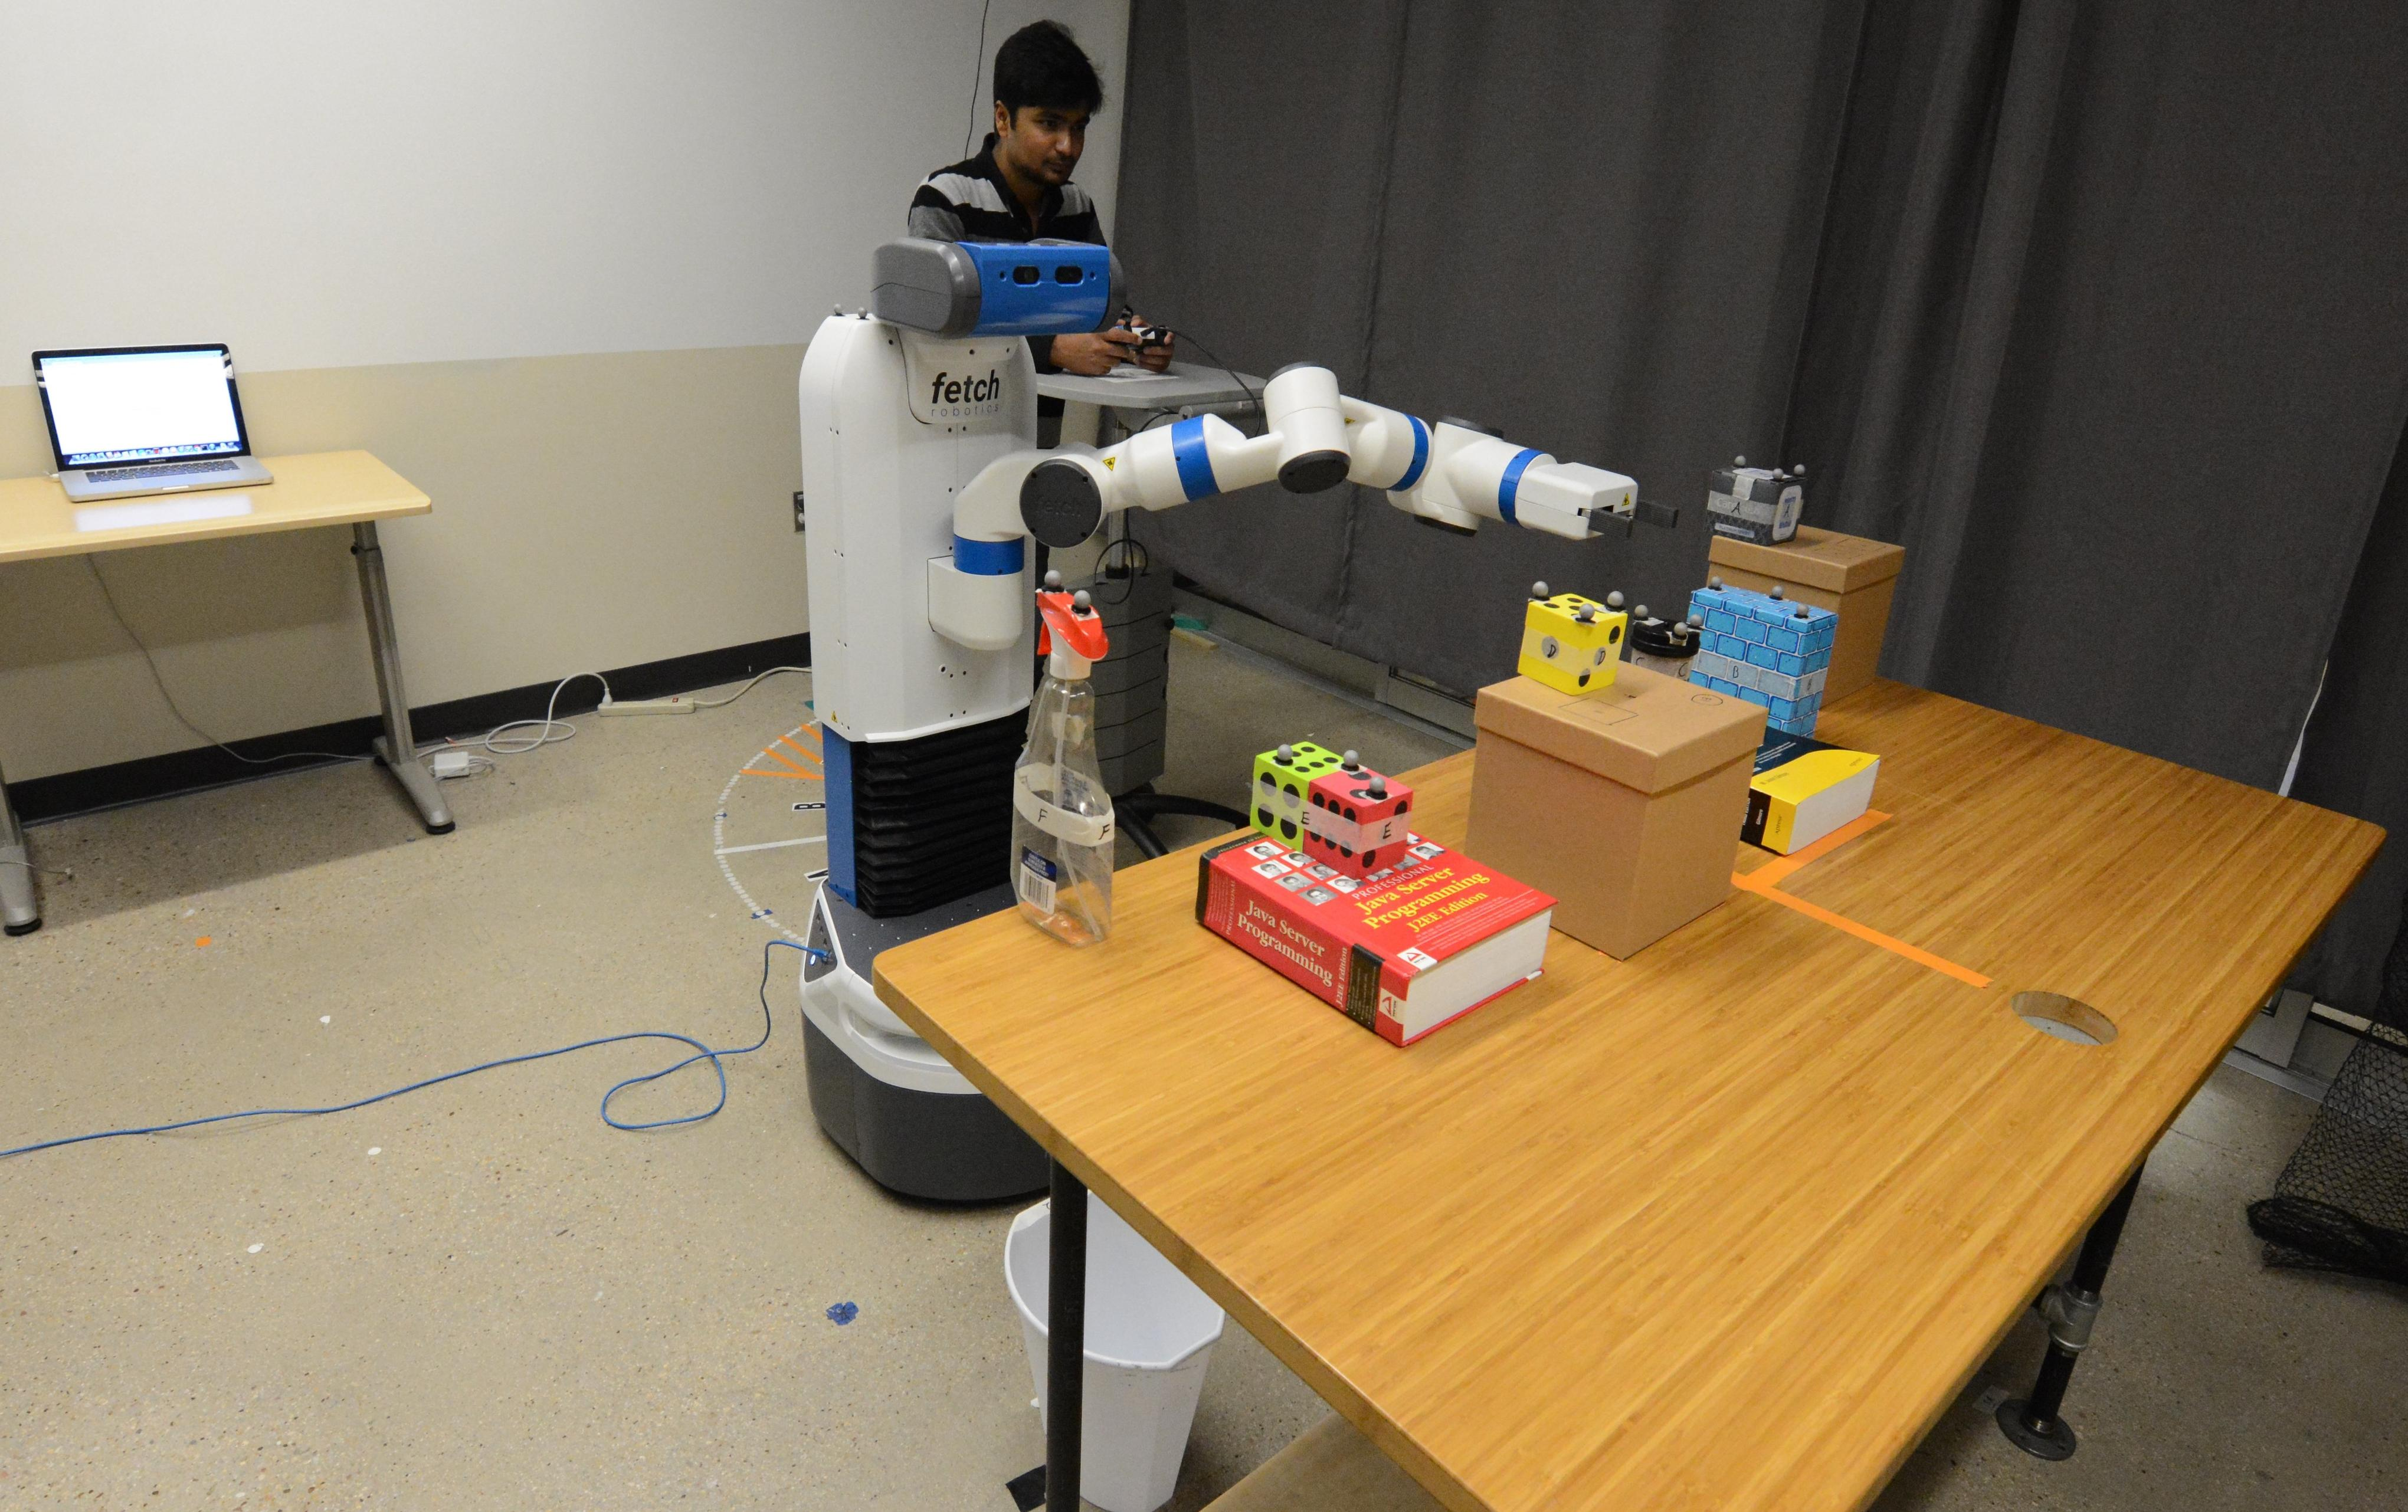
\includegraphics[width=0.49\columnwidth]{figures/task_setup-v3.jpg}
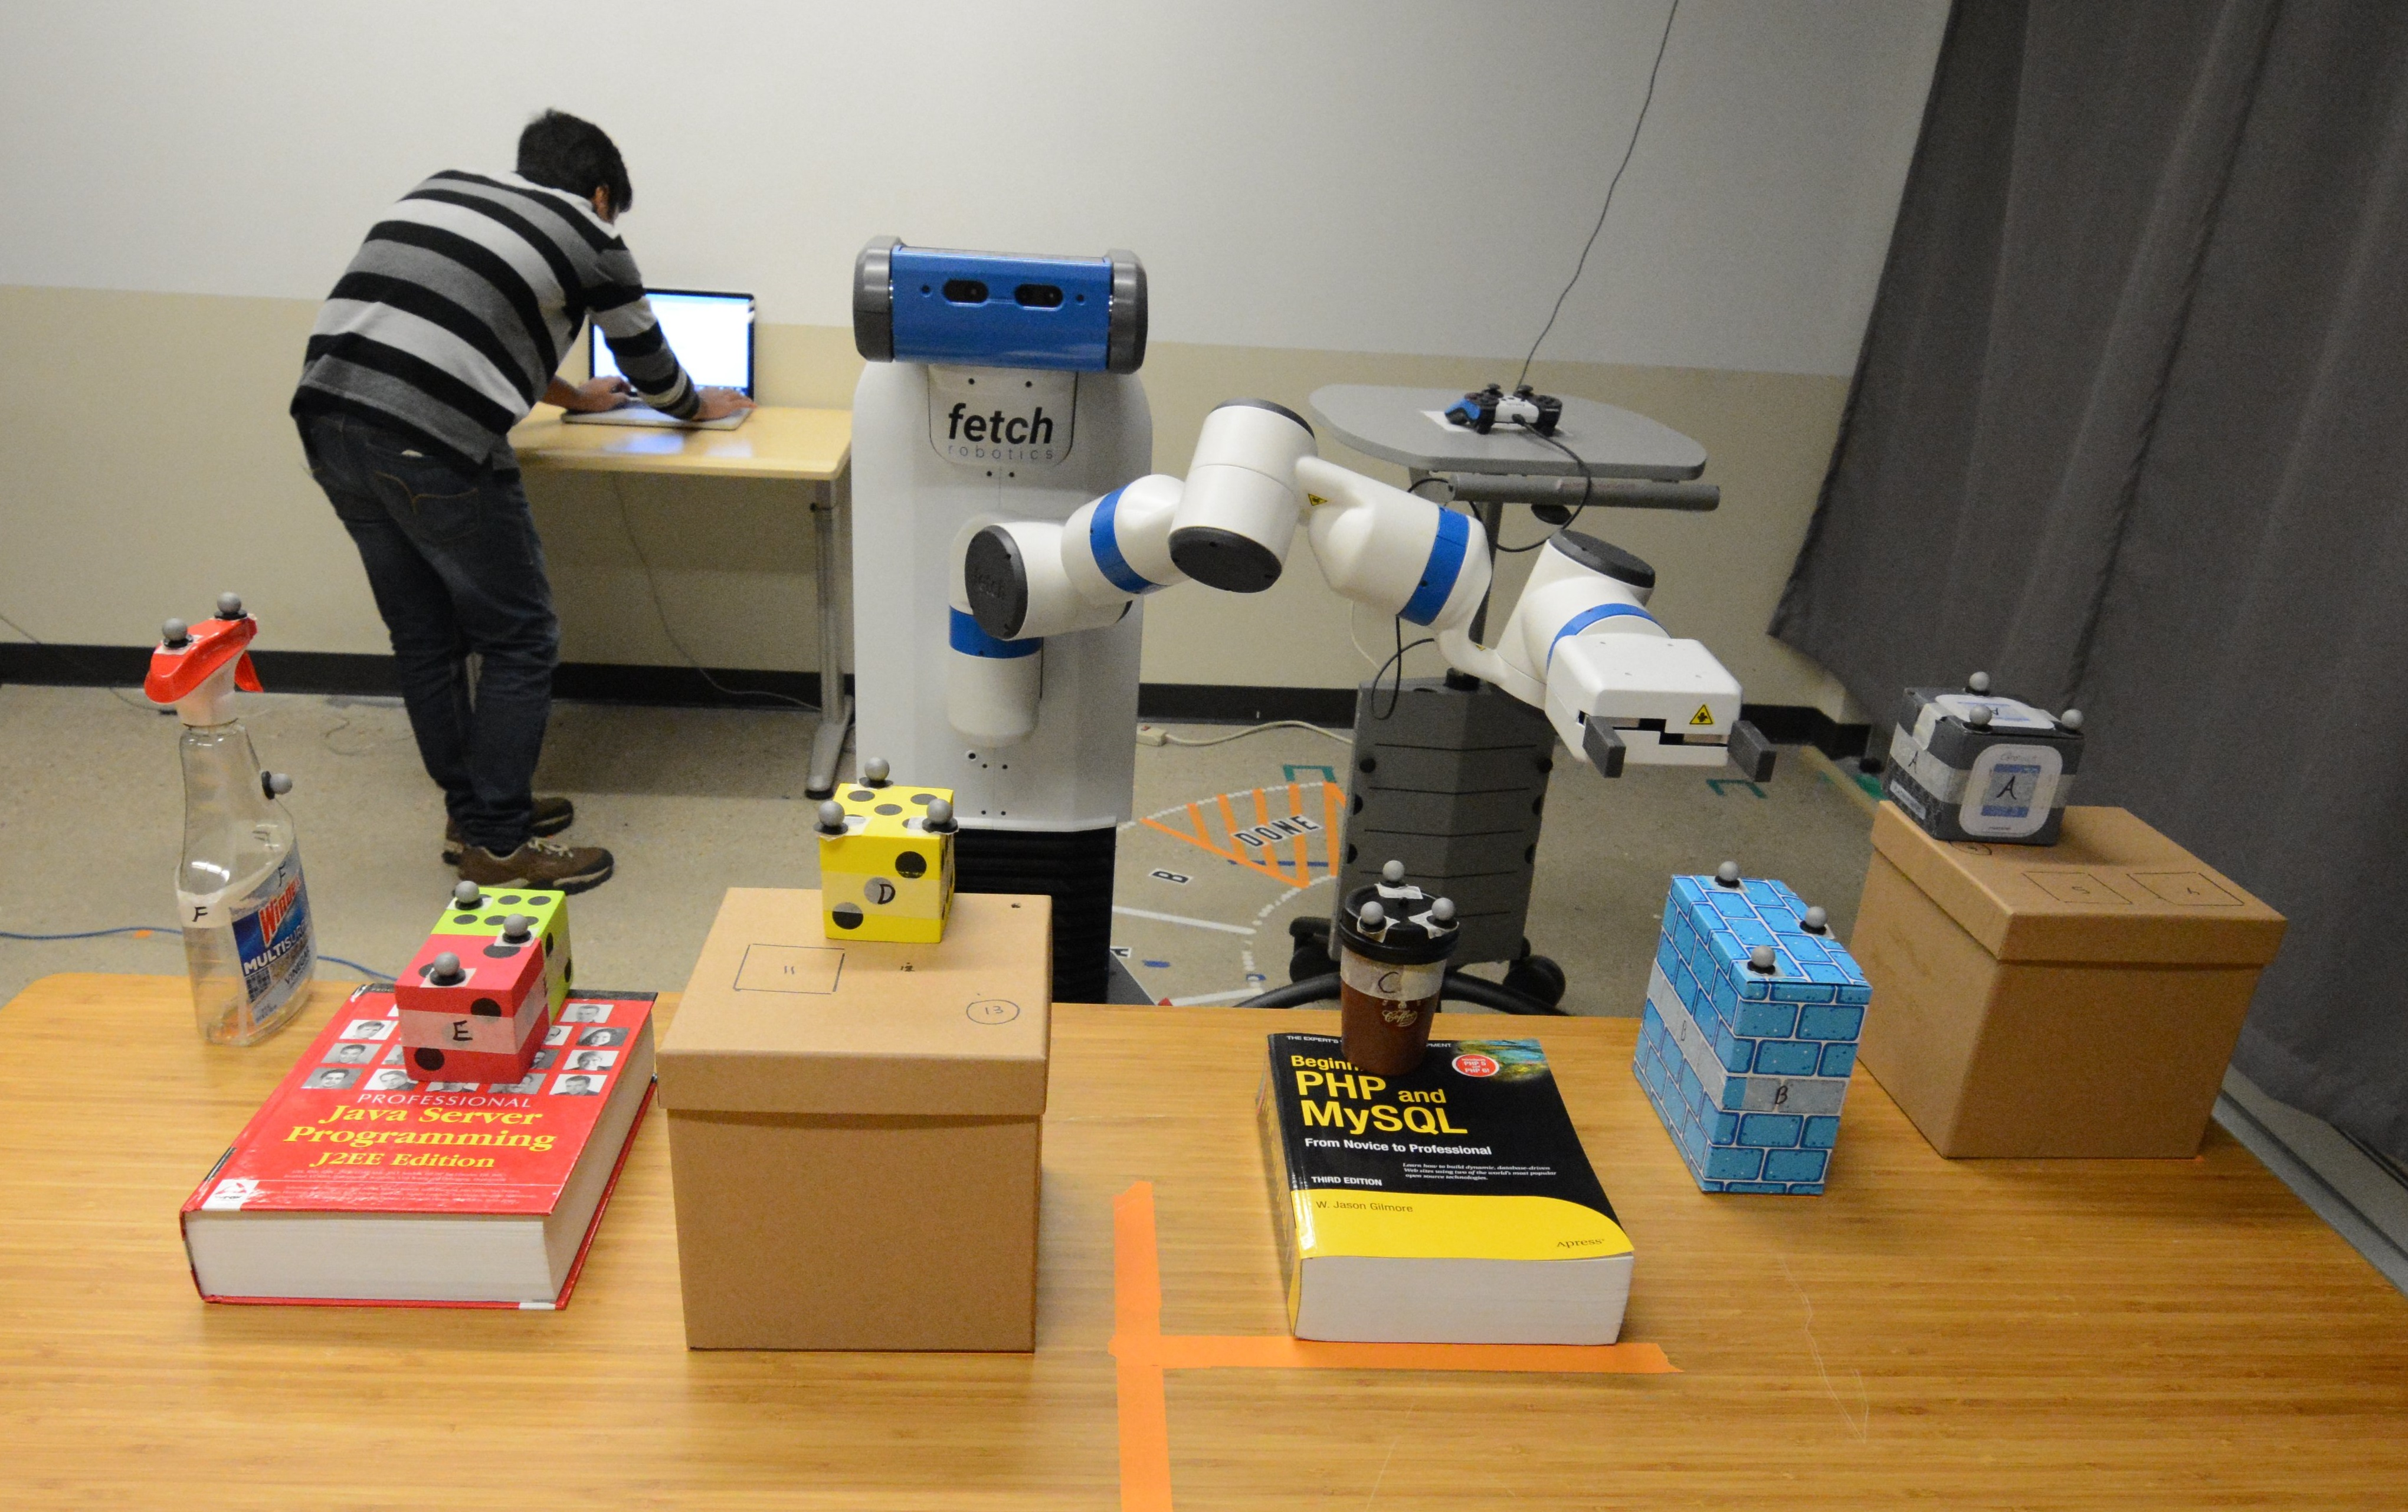
\includegraphics[width=0.49\columnwidth]{figures/teaser-v2.jpg}
\caption{A participant controls a robot during a multitasking user study. As the participant switches between tasks of actively inputting controls (left) and recording data on a laptop (right), the shared autonomy system provides assistance by continuing controls while the user is temporarily absent.}
\label{teaser}
\end{figure}

To improve system performance in a framework where the system learns from observed user actions, there are two distinct framework factors that can be manipulated: (1) the model of how the system learns from user actions and (2) what user actions are observed (i.e., \textit{active learning}). In this paper, we investigate active learning through information gathering actions within a shared autonomy paradigm. Our approach prioritizes robot configurations based on the amount of information the robot expects to gain from the user when user actions are next observed. The user changes nothing about their behavior and still provides the same implicit cues (control inputs), but information is gained more rapidly through exploiting areas where the inferred internal policy of the user is maximally different for different candidate goals. We refer to this strategy of moving toward information-rich states as \textit{information gathering actions}, which contrasts with purely \textit{goal-oriented} actions that move the robot toward what are believed to be the user's current goals. In this paper, we create a system that balances information gathering and goal-oriented actions and explore its utility in a user study involving shared autonomy control for a multitasking user.

\section{Background}

Our approach draws on prior work from goal-oriented shared autonomy systems and research on active learning and information gathering.

\subsection{Goal Prediction in Shared Autonomy}

Prior research has investigated shared autonomy and assistive teleoperation in an effort to make robot teleoperation easier, safer, and more efficient. Early shared autonomy systems assumed that the robot would be given information about the current user goal or desired behavior, which was then used to determine assistance strategies that helped users accomplish their predefined goal \cite{aigner1997human, debus2001cooperative, goodrich2001experiments}. While systems relying on such knowledge can be efficient, we are interested in creating more fluid interactions that do not require the overhead of explicitly defining user goals.

More recent work in shared autonomy and assistive teleoperation has moved away from previously-held assumptions about explicit goal communication. To develop systems that do not need \textit{a priori} specifications of the user's goal, these systems rely on predicting user intent and using a distinct goal-oriented strategy that assists toward the currently predicted user goal \cite{dragan2012formalizing, fagg2004extracting, kragic2005human, schultz2017goal, yu2005telemanipulation}. This ``predict-first'' approach can provide more general assistance than systems in which a goal must be manually specified; however, one drawback is that the goal-oriented assistance is only available once the current goal has been predicted with sufficient confidence. This limitation motivates our work, in which we explore how to improve system learning of user goals.

To this end, our work builds upon and investigates new use cases for hindsight optimization approximations in selecting assistance actions. Hindsight optimization provides a framework for reasoning about shared autonomy assistance in the presence of multiple potential goals. For example, \citet{javdani2015shared} set up a partially observable Markov decision process (POMDP) and use QMDP approximation \cite{littman1995learning}, or hindsight optimization, to estimate the best robot action at each timestep. This approximation eliminates information gathering from the POMDP solution and results in system action selection that weights the assistance toward each goal by the current belief in that goal. By selecting actions that optimize based on the current belief state over all goals, such a system enables goal-oriented assistance without a required confidence level for prediction of the user's goal.

This method was tested on two different shared control teleoperation tasks during which both user and system-generated controls were passed to the robot, with results demonstrating significant improvements in efficiency for the hindsight optimization system over both pure teleoperation strategies and the previously mentioned predict-first strategies \cite{javdani2018shared}. While this is a promising approach to goal-oriented assistance, it does not utilize the potential for shared autonomy systems to explore the state space in order to better learn about the user's goals.

\subsection{Active Information Gathering over Human State}
Our novel shared autonomy system makes use of exploration by integrating robotic actions that actively gather information about human objectives. This concept follows work on active learning for designing queries in order to more efficiently learn from humans. For example, \citet{liu2017bignav} apply such a strategy in creating a system for user view navigation that outperforms traditional methods by displaying views to a user that maximize information gain. Their system uses principles of information gain to choose new views as a user navigates through a large multiscale interface in order to more quickly ascertain the user's ultimate intended view. Similarly, \citet{thomason2017opportunistic} apply active learning in selection of user queries to improve grounding of learned terms.

Our work is further inspired by the work of \citet{sadigh2016information}, which developed a system for an autonomous car that tests how human drivers react to certain ``probing'' actions of the autonomous car (e.g., starting to merge in front of a human driver) in order to glean information about some factor of the driver's internal state (e.g., a driver's aggressiveness). Their approach centers on using a reward function that minimizes the entropy of the belief state over human drivers' internal states. We apply this idea of choosing actions that minimize entropy in the belief state to shared autonomy, where the belief state is over user goals. Applying this active learning framework to shared autonomy introduces new challenges from autonomous driving, including the investigation of the effects of information gathering when the human and autonomous system have shared control of the agent (as opposed to distinct agents where the active learning autonomous system has full control of its agent), balancing information gathering and goal-oriented actions while providing useful assistance to a user, and evaluating human assessments of working with an active learning shared autonomy system. The work of \citet{landolfi2017exploring} investigates the theoretical application of active learning to shared autonomy using simulated human data, but does not combine learning with goal-oriented assistance. We extend this prior research by contributing a method for balancing information gathering and goal-oriented assistance in shared autonomy, data from a user study involving working with an active learning shared autonomy system on a physical robot, and results on shared autonomy in multi-tasking scenarios.

\subsection{Shared Autonomy for a Multitasking User}
We believe that use cases involving human teammates that are intermittently absent represent one promising class of scenarios where shared autonomy systems can prove useful. In this work, we focus on one such use case where a user is tasked with operating a robot while handling other periodic duties that cause them to relinquish robot control on a regular basis. In such scenarios, neglect tolerance, or the ability of human users to neglect the robot \cite{crandall2002characterizing, olsen2003metrics}, can provide a useful measurement regarding the capability of the robot's autonomy. The ability of the robot to carry on with its task while unsupervised allows human users to attend to other tasks, such as operating other robots \cite{crandall2005validating, cummings2008predicting}, conducting data analysis, or performing other essential operations. In this work, we investigate how shared autonomy systems might support human users in a task where users only have intermittent control of the robot and perform other tasks simultaneously (such as monitoring and logging sensor readings).

\section{Information Gathering in Shared Autonomy}\label{formulation}

In this section, we describe our formulation for active information gathering during shared autonomy. We use a similar formulation to that used in \cite{sadigh2016information, sadigh2018planning}, with the novel additions of entropy as a weighting factor to balance exploration and exploitation and a method for balancing learning with goal-oriented assistance and user controls.

\subsection{Formulation}

Let $ x \in X $ represent the system state. This could encompass just the robot joint position, a more involved model including physical constraints, or some other representation (in our implementation, state represented the position of the robot's end effector in 3D space and a momentum factor consisting of the currently active movement plan's direction). We assume that the user in our teleoperation system has a unique goal in mind, $\phi \in \Phi$. Actions are represented by $ u \in U $, including both actions input by the user or actions actuated by the robot. We use $u_H$ to denote user-input actions. We also assume access to a model of the system transition function, $T: X \times U \rightarrow X$.

\subsection{User Action Observation}
In order to use our observations of user actions at each timestep $u_H^t$ to update our estimate of $\phi$, we find the model of the user's reward function as parametrized by $\phi$ that best explains the observed user inputs. Other related research has used the principle of maximum entropy \cite{ziebart2008maximum} to create a model over trajectory probability distributions \cite{dragan2012formalizing, javdani2015shared}, while our approach uses a model over action probability distributions inspired by the approach introduced by  \citet{ramachandran2007bayesian} that has also been used for prediction of human action selection parametrized by potential goals \cite{fisac2018probabilistically}. We apply this simplification to action space instead of trajectory space because user input actions do not necessarily correspond to actions taken by the system, thus the state-user action pairs are not equivalent to a trajectory. With this in mind, we assume that the human optimizes based on individual input actions rather than over trajectories, since they do not have full control over the trajectory. Additionally, we do not assume that the goal positions are static; if goals move during execution, models built using action probability distributions are not affected since each action is parameterized by the current position of all possible goals. This simplification also allows us to compute the normalizing factor for our distribution analytically, as the action space is small and discrete, compared to using a continuous trajectory space, which would require us to estimate the normalizing factor \cite{javdani2015shared}.

We define a reward function $R_\phi (x, u)$ that estimates the value of choosing action $u$ in state $x$ while attempting to reach goal $\phi$, which is assumed to be fixed. This reward function could be defined based on important features such as distance to goal or could be learned from user observations. In this work, we use a reward function corresponding to the anticipated difference in distance to the goal before and after taking action $u$:
\begin{equation}
R_\phi (x, u) = dist(x, \phi) - dist(T(x, u), \phi)
\end{equation}
Similarly to \citet{ramachandran2007bayesian}, we use a Boltzmann distribution over reward to model the user's probability of choosing an action:
\begin{equation}
P(u_H|\phi, x) \propto exp(R_\phi (x, u_H))
\end{equation}
Since our action space is discrete, we are able to normalize using a summation over possible actions:
\begin{equation}
P(u_H|\phi, x) = \frac{exp(R_\phi (x, u_H))}{\sum_{u \in U} exp(R_\phi (x, u))}
\end{equation}

Given an observation sequence of states and user inputs, $\xi^T = \{(x^0, u_H^0), (x^1, u_H^1), ..., (x^T, u_H^T)\}$, we can then define the likelihood of this observation sequence for a given $\phi$ through the following equation:

\begin{equation}
P(\xi|\phi) = \prod_tP(u_H^t|\phi, x^t)
\end{equation}

This assumes that the user's policy is \textit{stationary}, i.e., it does not change through the course of the observation. Consequently, the individual action choices can be considered independent. We apply Bayes theorem to obtain our estimated likelihood of the goal given the current observations:

\begin{equation}
P(\phi|\xi) = \frac{P(\xi|\phi)P(\phi)}{\sum_{\phi' \in \Phi}P(\xi|\phi')P(\phi')}
\end{equation}

Since our \textit{a priori} distribution of goal states is uniform, we can simplify to obtain our final goal likelihood equation:

\begin{equation}
P(\phi|\xi) = \frac{P(\xi|\phi)}{\sum_{\phi' \in \Phi}P(\xi|\phi')}
\end{equation}

\subsection{Goal-Oriented Actions through Hindsight Optimization}

We incorporate goal-oriented actions into our system by including a scoring term that uses the hindsight optimization technique introduced by \citet{javdani2015shared} for estimating the state-action value function. Recall that $R_\phi(x, u)$ represents the state-action reward function for system state augmented by goal $\phi$. The basic approach of hindsight optimization involves estimating the reward for a state-action pair, $R(x, u)$, despite not knowing $\phi$, by summing over $\Phi$. This gives an estimate of the true state-action reward function (the reward function parameterized by the human's true goal) by weighting each goal according to the current belief state. Formally, let $b$ encode our belief state at time $t$:
\[
b_t(\phi) = P(\phi|\xi^t)
\]
We apply the hindsight optimization approximation to estimate the reward $R^{HO}$ for each state-action pair given the current belief state:
\begin{equation}
R^{HO}_{b_t}(x,u) = \sum_{\phi \in \Phi} R_\phi (x, u_H)b_t(\phi)
\end{equation}

\subsection{Expected Information Gain at a New State}

In order to quantify the value of the information gain expected from a state, we estimate the reduction in entropy of the current belief state that will result from observing an user action at that state. To do this, we use the Minimum Expected Entropy approach developed for active learning \cite{holub2008entropy}. Let the entropy over the goal belief after an observation sequence $\xi$ be given as follows:

\begin{equation}
H(\xi) = -\sum_{\phi \in \Phi} P(\phi|\xi)log_{|\Phi|}(P(\phi|\xi))
\end{equation}

Assume that a new state action pair is observed, $(x',u_H')$, creating observation sequence $\xi' = \xi \cup (x', u_H')$. The information gain $I$ from this new observation is the difference in entropy before and after the observation:

\begin{equation}
I(\xi, \xi') = H(\xi) - H(\xi')
\end{equation}

However, the difficulty in evaluating the information gain of a state is that $u_H'$ is unknown prior to visiting the state. To solve this, we follow the approach of \citet{holub2008entropy} by calculating the expected entropy through summing over the conditional entropies from all possible user actions at the state weighted by the likelihood of the user picking the action according to our current belief state about the user's goal, $b(\phi)$:

\[
\hat{H}(\xi, x') = \sum_{u \in U} P(u|b(\phi),x')H(\xi \cup (x', u))
\]
\begin{equation}\label{estimated_entropy}
= \sum_{u \in U} \sum_{\phi \in \Phi} P(u|\phi,x')P(\phi|\xi)H(\xi \cup (x', u))
\end{equation}

Using \eqref{estimated_entropy}, we can calculate the expected information gain of going to a new state $x'$:

\begin{equation}
\hat{I}(\xi, x') = H(\xi) - \sum_{u \in U} \sum_{\phi \in \Phi} P(u|\phi,x')P(\phi|\xi)H(\xi \cup (x', u))
\end{equation}

\subsection{Incorporating User and Robot Actions}
While we can pick actions that maximize $\hat{I}(\xi, T(x,u))$ in order to most quickly ascertain the user's goal, or actions that maximize $R^{HO}$ in order to optimize assistance, these strategies may result in the system choosing actions that are dramatically opposed to the user's inputs, potentially creating a frustrating user experience. Accordingly, we incorporate $D_{u_H}(u)$ into our framework as a function that penalizes actions far from those input by the user. Possible implementations for $D_{u_H}(u)$ could penalize actions based on the distances between either the two control vectors or the expected resulting states from applying the two control vectors. We include $D_{u_H}(u)$ for complete description of our framework, but in our experimentation, we constrained robot actions to follow user actions when given and did not apply this penalty at timesteps in which the user did not provide input. Thus, our experimental results do not demonstrate the effects of such a penalty term, and we leave the evaluation of the blending of user and system actions during information gathering for future work.

\subsection{Balancing Actions}

We modulate the weighting of information gathering actions and goal-oriented actions by the current entropy in the system: if entropy is high, information gathering actions are more likely to be taken than goal-oriented actions, and if entropy is low, goal-oriented actions are more likely to be taken than information gathering actions. We accomplish this by weighting both $\hat{I}$ and $R^{HO}$ by functions of our current entropy, $f_1$ and $f_2$ respectively. In our implementation, we use simple piecewise functions:
\[
f_1(H) =
\begin{cases}
H & H\geq 0.1 \\
0.1 & H < 0.1
\end{cases}
,f_2(H) = \frac{1}{f_1(H)}
\]
We incorporate a function of entropy as a weighting factor in our framework rather than using a simple linear combination in order to address the problem of exploration vs exploitation. As entropy varies with goal confidence, our approach handles exploration vs exploitation by balancing learning and assistance according to goal confidence.

This gives us three factors to determine the value of a candidate action: the expected information gain weighted by the current entropy, the movement toward the expected goal weighted by the inverse of the current entropy, and the distance between the candidate action and the user input. We also add tuning parameters $\alpha$, $\beta$, and $\gamma$ to adjust the magnitude of each factor. Combining all the tuning parameters gives us our weight vector $\theta = [\alpha f_1(H), \beta f_2(H), \gamma]$ that we use in order to perform action selection.

\[
u^* = argmax_u [ \theta \cdot [\hat{I}(\xi, T(x,u)), R^{HO}(x,u,b_t), D_{u_H}(u)]^T ]
\]

\subsection{Behavior}

To help visualize the differences in behavior between information gathering actions and goal-oriented actions based on hindsight optimization, Fig. \ref{heatmap2} illustrates a heatmap produced from multiple candidate goals, scoring each state according to either expected information gain or goal-oriented reward (for visualization purposes Fig. \ref{heatmap2} was created by discretizing a 2D space, although our system implementation actually operated with goals in continuous 3D space). In this figure, goals A and B are believed to be more likely than the other goals. Both goal-oriented and information gain scoring reward states closer to the more likely goals, but goal-oriented scoring is much more aggressive with respect to rewarding the positions closest to the two most likely goal candidates.

\begin{figure}
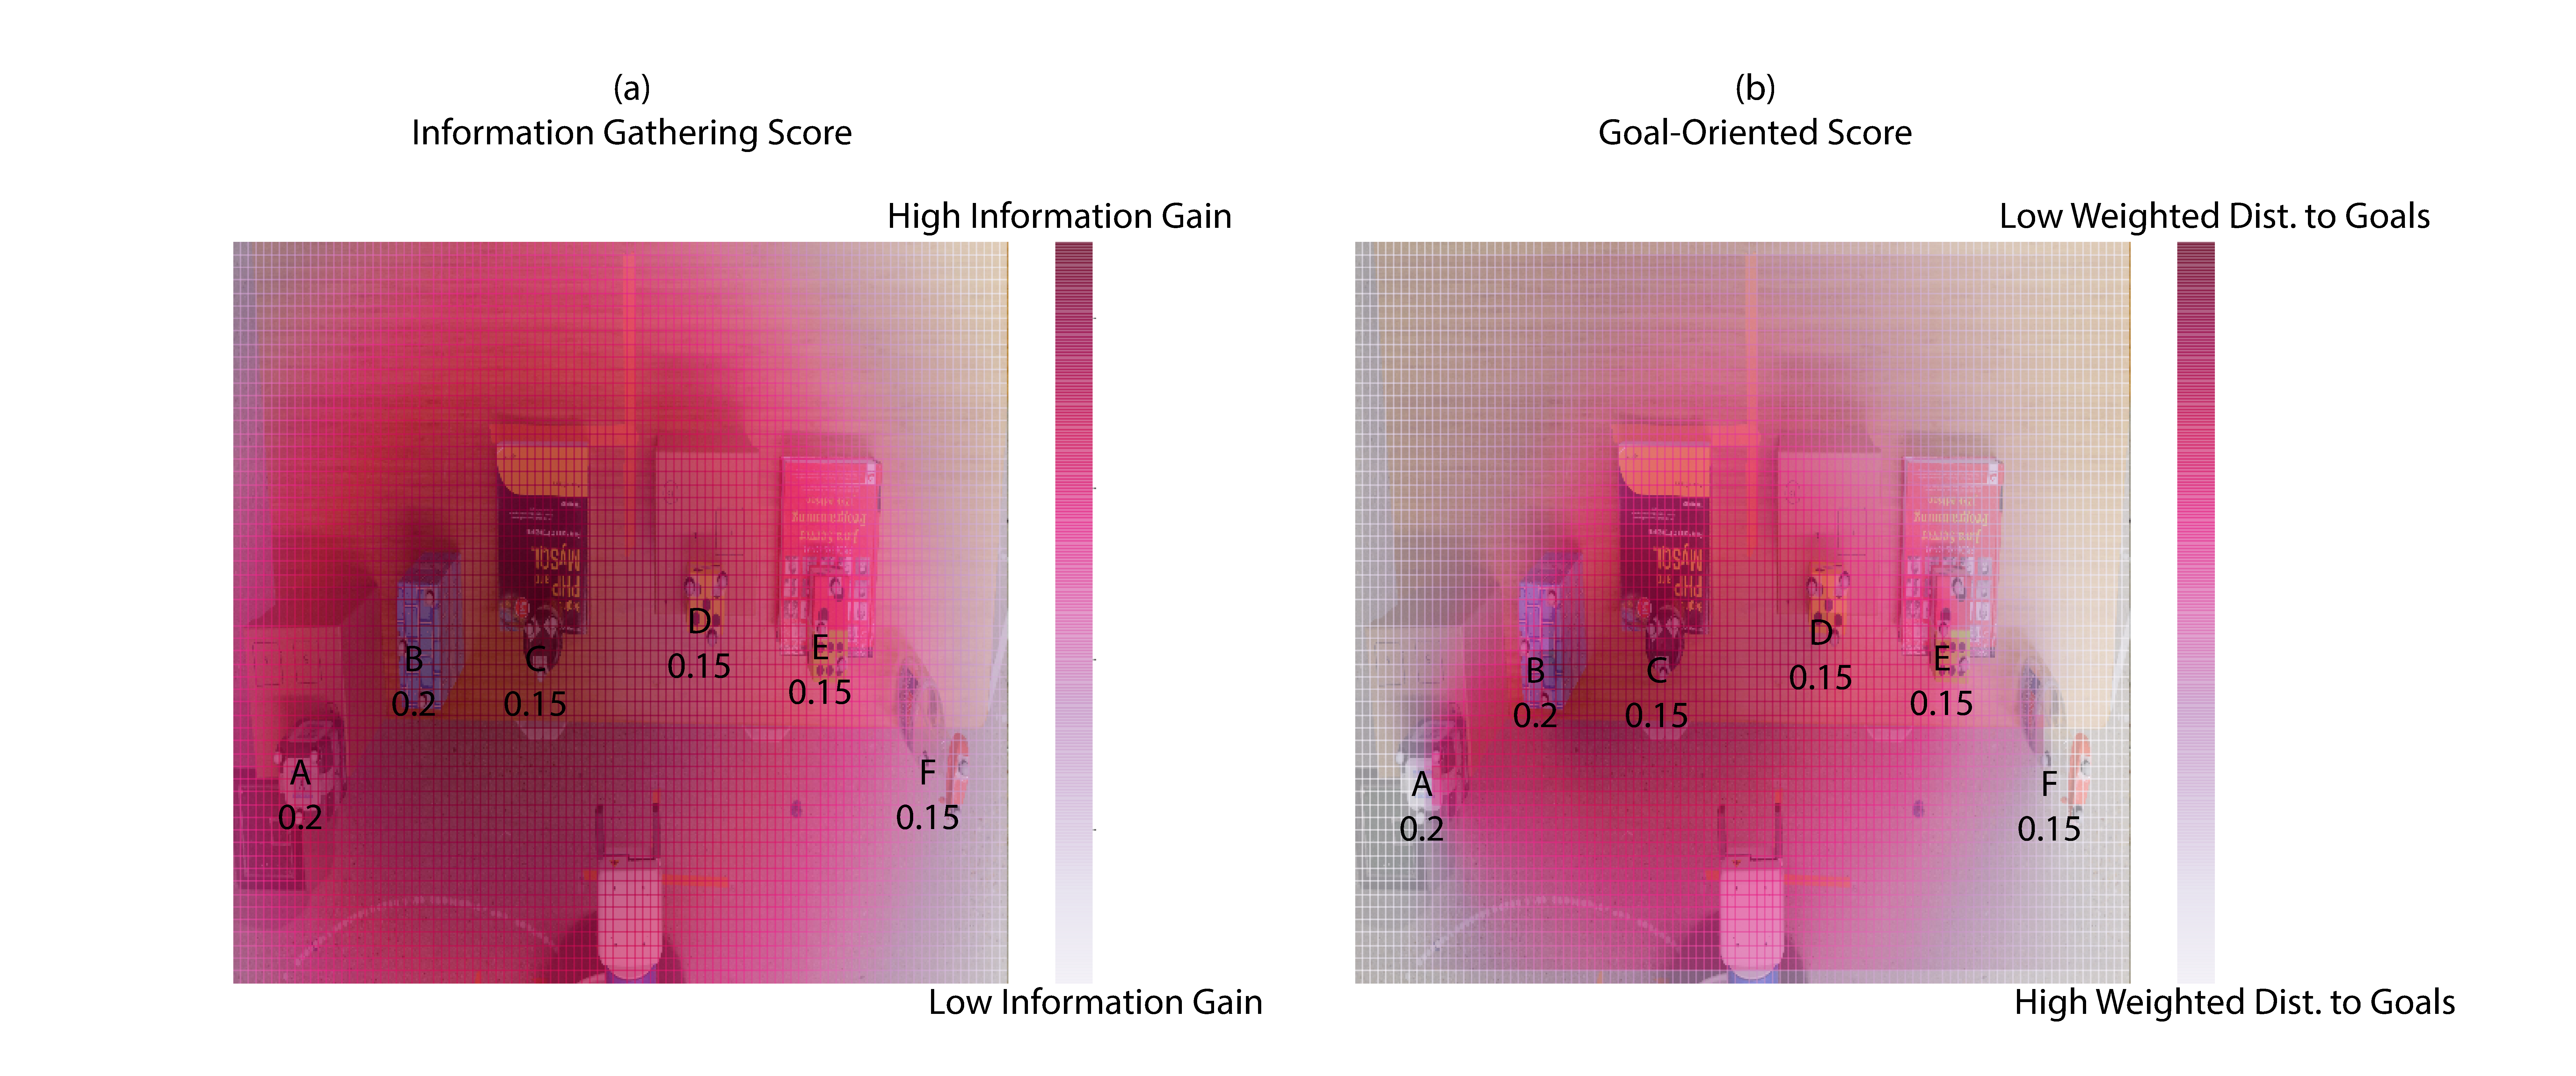
\includegraphics[width=\columnwidth]{figures/Heatmap_Uneven_Belief.pdf}
\caption{Heatmap of expected information gain by state (A) compared to heatmap of hindsight optimization's goal-oriented reward (B) in which goals have different probabilities.}
\label{heatmap2}
\end{figure}

\section{Experimental Evaluation}

We conducted an in-person laboratory experiment to investigate differences in user multitasking scenarios between pure teleoperation, goal-oriented shared autonomy via hindsight optimization, and balanced information gathering shared autonomy.

\subsection{System Implementation}\label{implementation}
In order to demonstrate our shared autonomy system and evaluate the effects of information gathering and hindsight optimization during user multitasking, we created a system for controlling the end effector of a Fetch robot. We created this control system such that joystick controls on a Playstation 3 controller mapped to directions in Cartesian space, and two separate buttons could be pressed to open and close the end effector. Directional controls were discrete, with three possible controls for each axis (i.e., forward, no movement, and backward), and directional controls for each of the three axes could be combined to move diagonally. This created 27 possible directional control actions at each timestep.

In our implementation, no direct manipulation of the pose of the end effector was involved in the control system, and all end effector movements followed Cartesian paths generated by MoveIt \cite{sucan2013moveit} with a max step size of 5 cm between end effector configurations, creating smooth and linear movement of the end effector. We chose to create this simplified, linear control system instead of using direct manipulation over the robot's 7-DOF arm in order to make the controls quick to pickup and the robot's movement easy to understand for novice users (pretests of an earlier version of our system showed that novice users had significant trouble operating the joints directly). Our shared autonomy system used the same set of directional controls as that provided to the user.

Control updates occurred at a rate of 2 Hz to ensure that every action had visible effects (i.e., visible robot movement), even after including the motion planning delay and robot joint acceleration. We also chose to prevent the robot from overriding participant controls in this study, which was accomplished by setting an arbitrarily high value for $\gamma$, the tuning parameter that adjusts the acceptable distance between user input and system output. While we believe that there are many interesting questions to address about interweaving these control systems with active human controls, we constrained the scope of our study to focus specifically on the impact of information gathering and goal-oriented actions for multitasking users through using these systems to take over only during timesteps with no user controls. We chose tuning values for $\alpha$ and $\beta$ (the tuning parameters for information gathering and goal-oriented actions, respectively) to keep the order of magnitude the same for the reward from information gathering actions and goal-oriented actions, such that information gathering actions were weighted higher than goal-oriented actions with high entropy (e.g., $H > 0.7$), and goal-oriented optimization actions became dominant with low entropy (e.g., $H < 0.3$).

\subsection{Experimental Design}

We ran a $3 \times 1$, within-participants user study ($N = 12$, 9 male and 3 female) that compared three teleoperation control systems: pure teleoperation,  goal-oriented shared autonomy (via hindsight optimization), and balanced information gathering. The control systems were setup as follows:

\subsubsection{Pure Teleoperation}
In this condition, the robot did not take any actions when the participant was not actively sending controls. Belief updating was still done for analysis purposes, but the belief state was not used in any way by the robot.
\subsubsection{Goal-Oriented}
In this condition, $\alpha$ was set to 0, causing the hindsight optimization-based goal-oriented reward to be the only factor when choosing actions during timesteps with no participant control inputs.
\subsubsection{Balanced Information Gathering}
In this condition, the full system was used for choosing actions, including both goal-oriented and information gathering factors.

Participants completed three trials, using a separate control system for each trial. Each trial consisted of participants operating the robot to move three of six objects from a table to two bins on the floor, as seen in Fig. \ref{teaser}. Participants were given ordered instructions by the experimenter of which object to grab and the bin to which that object should be moved. After each object was dropped into a bin, the arm reset itself to its starting position. This effectively created six tasks per trial: three ``pickup" tasks and three ``dropoff" tasks. The context participants were given was that of cleaning up after a ``chemical spill", requiring the robot to dispose of the objects.

While participants operated the robot, they were also required to monitor a laptop approximately 2 meters away that would periodically receive new ``sensor readings" (see Fig. \ref{teaser}). New sensor readings were signified by loud audio alerts. The readings started 10 seconds into the trial, and repeated every 20 seconds after that until the trial was completed. Participants were instructed to log each sensor reading within 20 seconds of each alert, before a new reading appeared. Logging the sensor readings required setting down the controller for the robot, which was attached to the robot control station (see Fig. \ref{teaser}). This forced the participants to multitask between operating the robot with the controller and logging sensor readings on the laptop. This also forced regular interruptions of participant control inputs, during which time the different conditions affected how the robot behaved.

Each participant completed six tasks per condition, for a total of 216 tasks (72 tasks per condition). We counted pickup tasks as a success if the participant was able to successfully grab and move an object, and we counted dropoff tasks as a success if the participant was able to move the object above the bin and drop it such that it fell either in the bin or within 10 cm of the edges of the bin.

We took several steps to mitigate potential ordering effects that might arise due to our within-participants design. Our simplified linear robot control system (rather than direct 7 DOF control) was designed to be simple enough that participants could rapidly become proficient, rather than learning and improving across trials. We also had a brief practice period before each trial during which participants operated the robot using the control system that they would be using in the upcoming trial. This practice period involved grabbing a single object (separate from those used for goals in the experiment) and moving it on the table, and ended once the participant was able to successfully grab, move, and drop the object (this practice period typically lasted less than a minute). We fully counterbalanced condition order to further mitigate any remaining ordering effects. Goals and ordering of goals for object pickup and dropoff were fully randomized, as were the values of the ``sensor readings" (although the timing for the sensor readings was constant for all trials). After each trial, participants completed a survey regarding their subjective impression of that trial's control system.

During the experiment, positions of all object goals and dropoff goals were provided to the robotic system by a VICON motion capture system. The system also switched between two different goal sets depending on the status of the gripper: when the gripper was open, the system used the positions of the objects to be picked up as candidate goals, and when the gripper was closed, the system used the positions of the dropff bins as candidate goals. Each time an object sorting task was completed, that object was removed from the system's list of candidate goals and the system's belief state and recorded human action observations were reset.

\subsection{Measures}

Based on the differences in our control systems, we expected to see differences in the belief state updating, task efficiency, and subjective user experience. We used several objective and subjective measures to assess the performance of the pure teleoperation, goal-oriented, and balanced information gathering systems. In analyzing our results, we examined the individual \textit{pickup tasks} and \textit{dropoff tasks} completed by participants (3 of each per trial).

\subsubsection{Objective Measures}
To evaluate the objective impacts of the control systems, we looked at overall \textit{total task efficiency} (number of combined user actions and autonomous system actions or inactions taken before task completion), \textit{belief convergence speed} (the number of user actions observed before the correct goal became the system's most likely goal for the remainder of the task), and behavior around \textit{shared autonomy windows}. Shared autonomy windows were any sequence of timesteps in which the participant did not input controls for at least 5 continuous timesteps, or 2.5 seconds. As the shared autonomy systems only affected the control of the physical robot while participants were not sending controls, these windows were the times during which the experimental conditions affected the robot's behavior. We chose a minimum of 5 continuous timesteps to use for analysis in order to ensure that short windows during which the control system would not have sufficient time to move the arm were not counted in our analysis. In order to ensure that homogeneity of variance held for this measure, we analyzed the total number of shared autonomy windows divided by the total control timesteps per condition, separated out by participant, giving us a measure of the window rate (the rate at which shared autonomy windows occurred). We found no significant difference between the window rate in goal-oriented ($M = 0.025, SD = 0.004$), balanced information gathering ($M = 0.025, SD = 0.002$), and pure teleoperation ($M = 0.025$, $SD = 0.002$) conditions.

\subsubsection{Subjective Measures}

We used a survey administered after each trial to measure subjective participant experience across each condition. Our survey used modified System Usability Scale (SUS) and NASA TLX scales with 7-point Likert-style questionnaire items for consistency between scales. These scales measured the \textit{usability} of each system and \textit{workload} caused by operating each system, respectively.

%
%\begin{figure}
%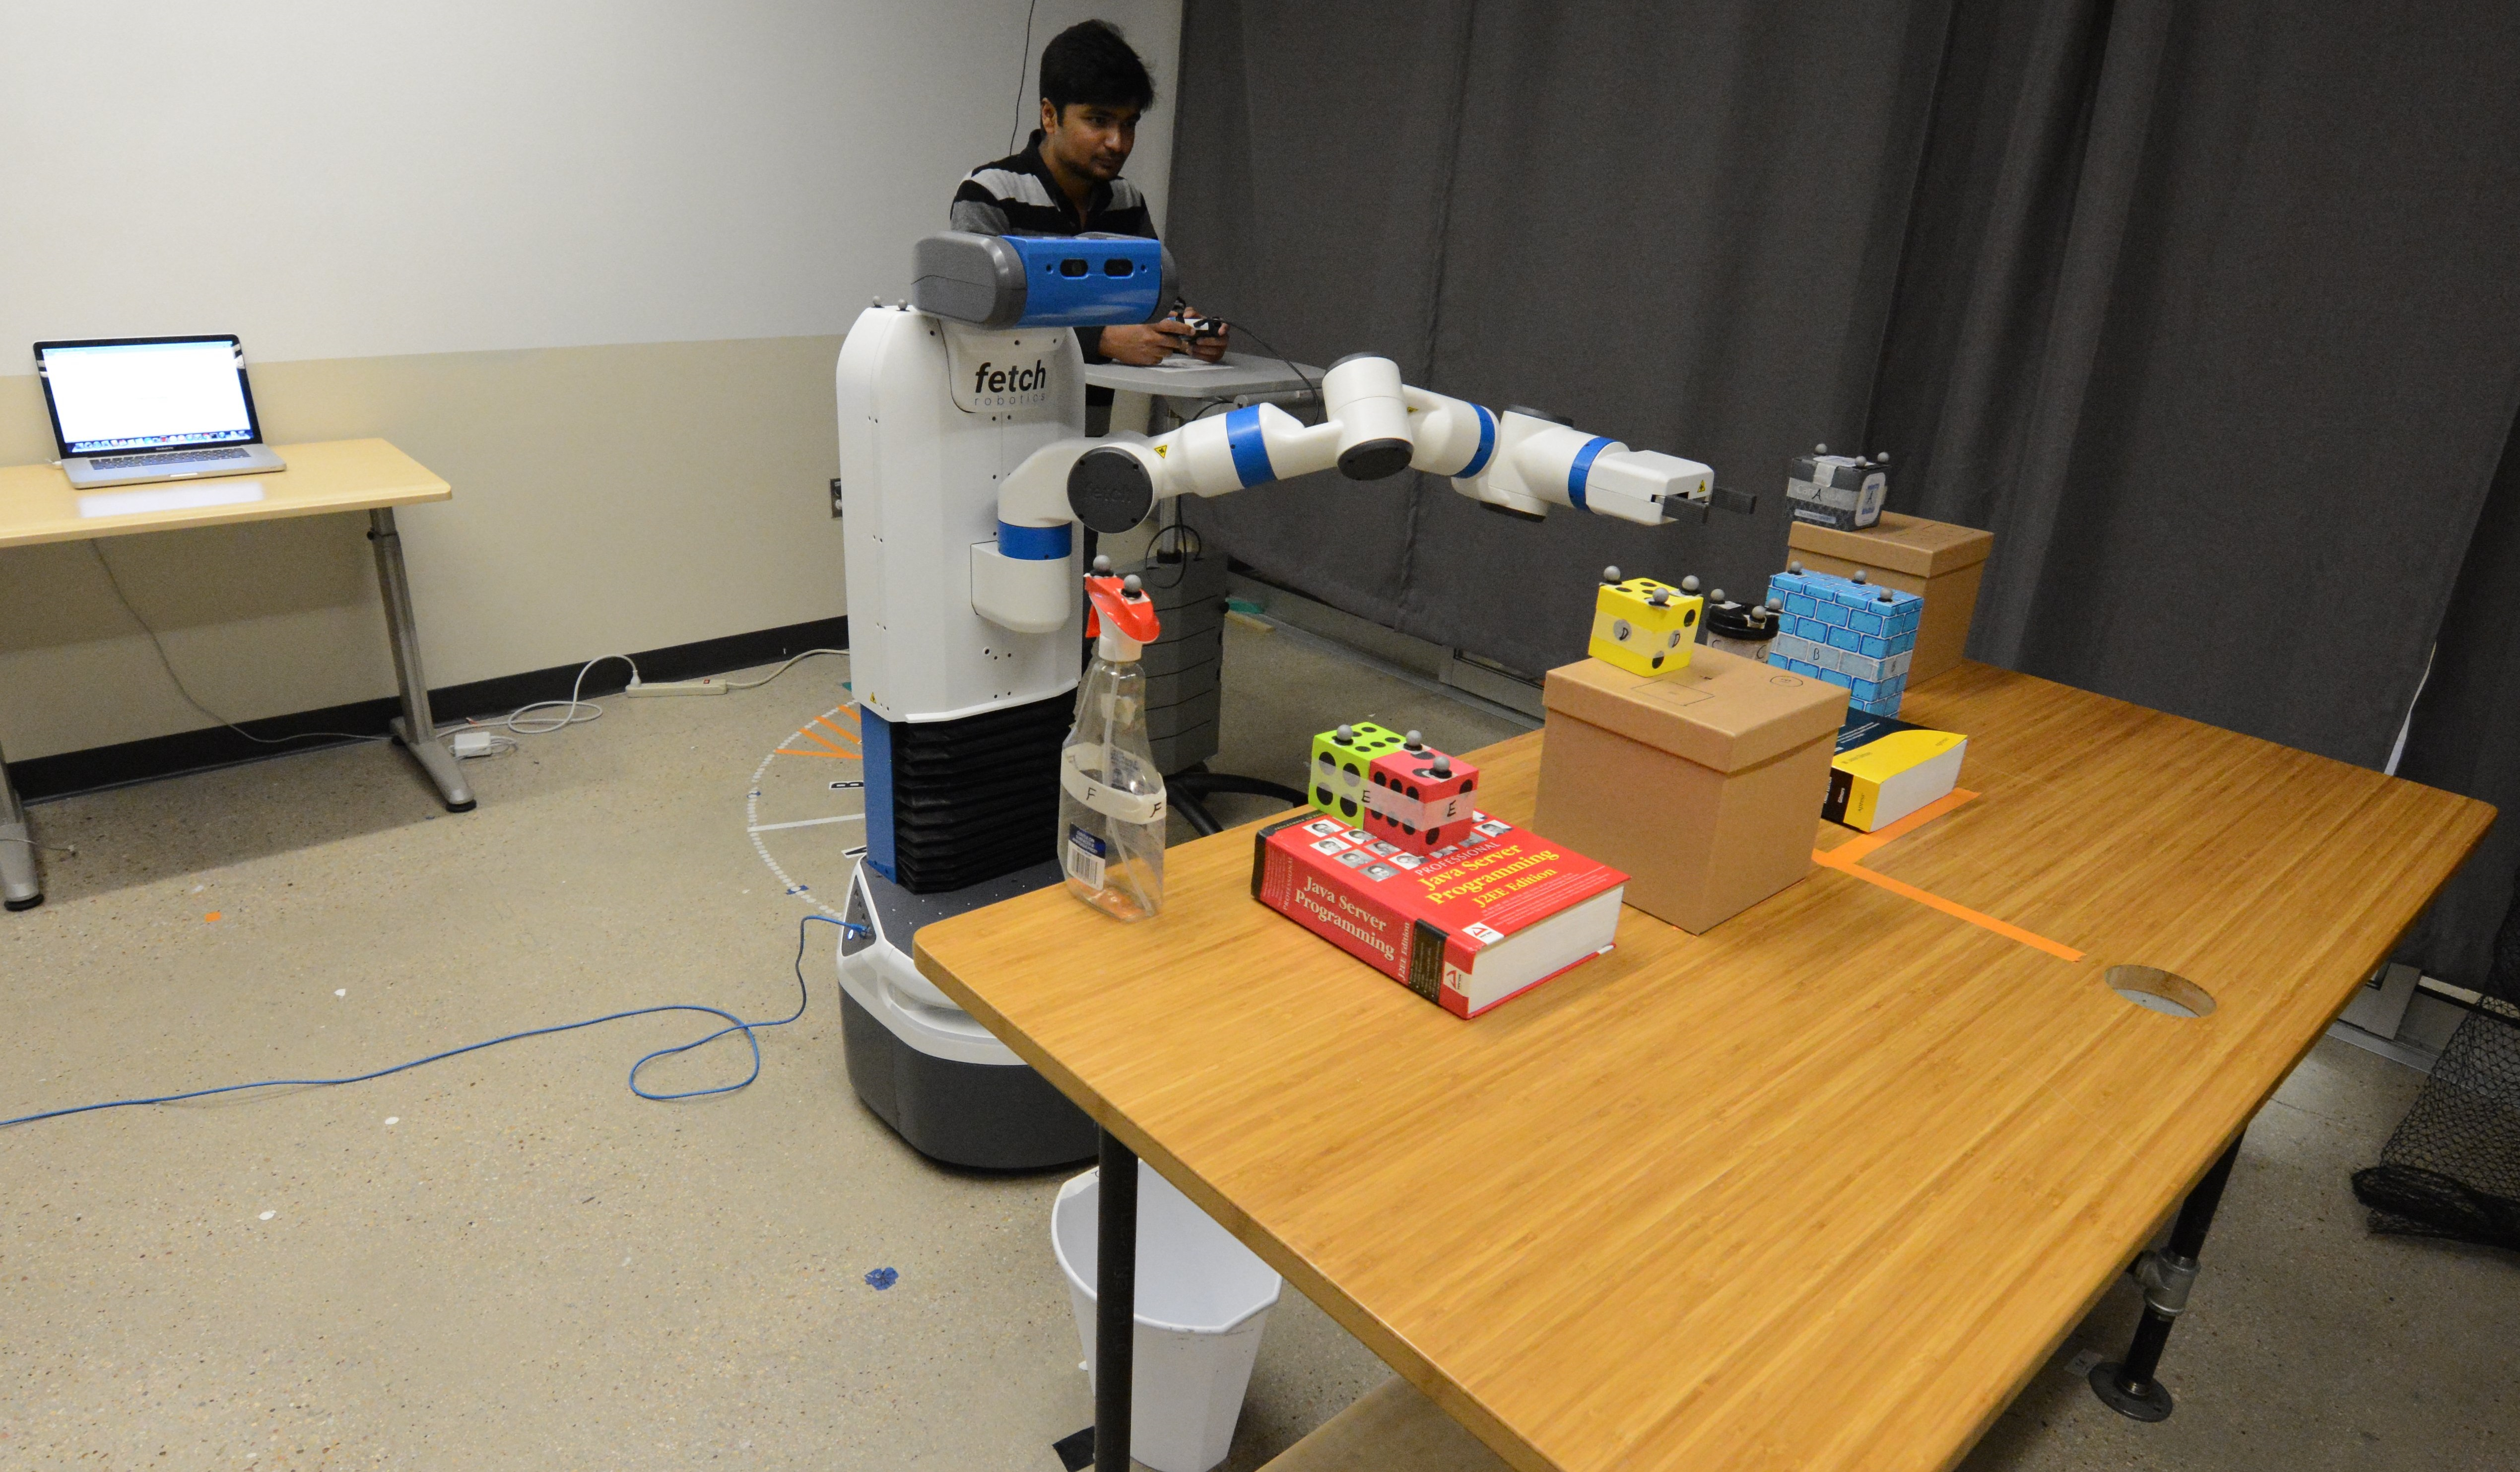
\includegraphics[width=\columnwidth]{figures/task_setup-v2.jpg}
%\caption{Experiment Setup}
%\label{exp_setup}
%\end{figure}
%

\section{Analysis and Results}

We found several differences between our conditions in aspects of robot behavior and task efficiency. These differences were found both in qualitative observations and further analysis of the data from our study.

\begin{figure*}
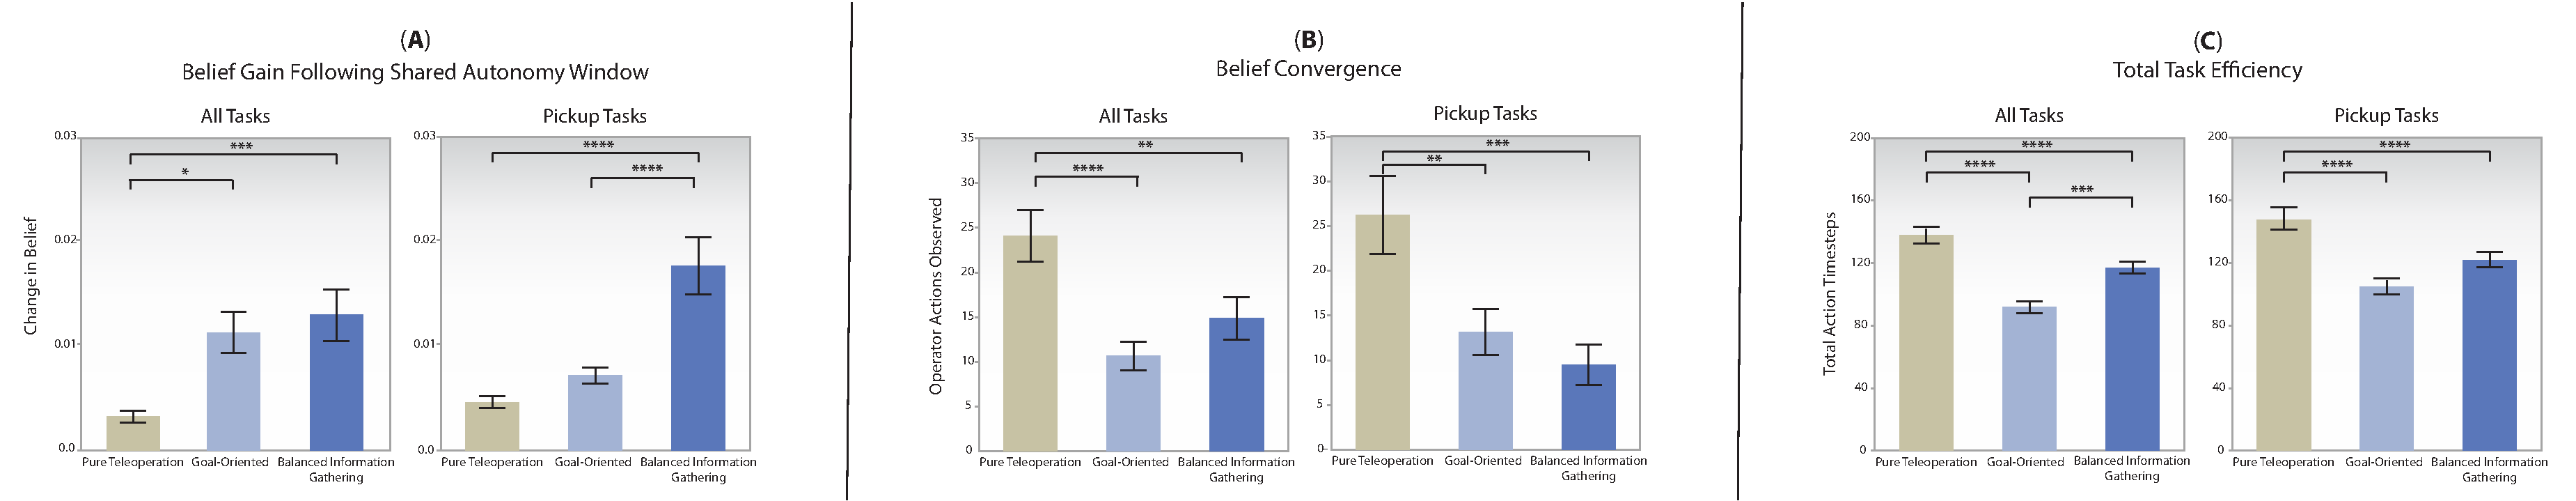
\includegraphics[width=\textwidth]{figures/CR_All_Measures.pdf}
\caption{The results from our objective measures show tradeoffs between the systems. The balanced information gathering systems provides significant improvements in belief gain after shared autonomy windows for pickup tasks (A). The balanced information gathering and goal oriented systems perform similarly for belief convergence while both outperform pure teleoperation (B), and the goal oriented system performs best in terms of total task efficiency for all tasks (C). *$= p < .05$, **$= p < .01$, ***$= p < .001$, ****$= p < .0001$.}
\label{picture_results}
\end{figure*}

\subsection{Observations}
There was only one failure during a pickup task (balanced information gathering condition), which occurred when a participant knocked over a goal object (a Windex bottle) while attempting to grab it. This task data was still used for analysis as the arm still went through the full trajectory for grabbing the correct goal and only failed during the gripping movement. However, the dropoff task data that would have followed this pickup task was not used due to there being no dropoff task since the pickup failed. There were three total failures during dropoff tasks, two of which (one goal-oriented and one balanced information gathering conditions) occurred with the same grasped object (the same Windex bottle) slipping out of the gripper during movement toward the bin, and one (balanced information gathering condition) which occurred due to the participant dropping the object at the wrong bin mistakenly. These three tasks were not included in the rest of the analysis as they did not include full trajectories of participant control toward the correct goal.

Qualitatively, we noticed a large difference in the behavior of balanced information gathering between the pickup and dropoff conditions, where it was evident that the balanced information gathering condition was much more successful at converging to the correct belief in pickup tasks than in dropoff tasks. Because of this, we completed analysis on the results from all tasks as well as the results from pickup tasks alone.

\subsection{Analysis}

We analyzed the data from our objective measures using a one-way analysis of variance (ANOVA) with experimental condition as a fixed effect and condition order and task goal as random covariates. As described above, we analyzed performance across pickup tasks alone and across all tasks (pickup and dropoff) as we noticed a difference in the impact of the balanced information gathering condition between pickup and dropoff tasks during qualitative observations. Finally, we analyzed the results from the two scales within our participant survey separately using one-way ANOVA tests with the experimental condition as a fixed effect.

\subsection{Objective Results}

\subsubsection{Belief Accuracy Gain after Shared Autonomy Windows}
We calculated the gain in belief accuracy that occurred during the next timestep once the participant resumed control after a shared autonomy window in order to evaluate how the robot's behavior during the shared autonomy window influenced the information that the system gained once the participant returned. We looked at all shared autonomy windows during which the entropy was higher than a threshold of 0.7, chosen due to this being the approximate value above which information gathering actions were dominant over goal-oriented actions based on our system tuning, as described in \S\ref{implementation}. For all tasks, we found a significant effect of condition on belief accuracy gain, $F(2, 244) = 7.72$, $p < .001$. Post-hoc comparisons using Tukey's HSD test revealed that both balanced information gathering ($M = 0.013$, $SD = 0.023$) and goal-oriented ($M = 0.011$, $SD = 0.017$) significantly outperformed pure teleoperation ($M = 0.003$, $SD = 0.005$) in terms of belief accuracy gain at significance levels of $p < .001$ and $p < .05$, respectively, but were not significantly different from each other. For pickup tasks alone, we also found a significant effect of condition on belief accuracy gain, $F(2, 105) = 16.57$, $p < .0001$, with Tukey's HSD test showing significant differences of balanced information gathering ($M = 0.018$, $SD = 0.017$) over both goal-oriented ($M = 0.007$, $SD = 0.005$) and pure teleoperation ($M = 0.005$, $SD = 0.004$) at significance levels of $p < .0001$,  and no significant difference between goal-oriented and pure teleoperation. These results are shown in Fig. \ref{picture_results} (A).

\subsubsection{Belief Convergence Speed}

We observed nine tasks (two pure teleoperation, three balanced information gathering, and four goal-oriented) which ended before the correct belief had become dominant; these trials were not included in the analysis. After analyzing all other tasks, we found a significant effect of condition on belief convergence speed, $F(2, 174) = 13.22$, $p < .0001$. Post-hoc comparisons using Tukey's HSD test revealed significant differences between balanced information gathering ($M = 14.85$, $SD = 19.13$) and pure teleoperation ($M = 24.11$, $SD = 24.07$) at a significance level of $p < .01$ and between goal-oriented ($M = 10.64$, $SD = 13.17$) and pure teleoperation ($p < .0001$), but not between balanced information gathering and goal-oriented. For pickup tasks alone, we found a significant effect of condition on belief convergence speed, $F(2, 87) = 9.52$, $p < .001$. Post-hoc comparisons using Tukey's HSD test again revealed significant differences between balanced information gathering ($M = 9.53$, $SD = 13.48$) and pure teleoperation ($M = 26.22$, $SD = 26.09$) at a significance level of $p < .001$ and between goal-oriented ($M = 13.14$, $SD = 15.15$) and pure teleoperation ($p < .01$), but not between balanced information gathering and goal-oriented. Fig. \ref{picture_results} (B) visualizes these results.

\subsubsection{Total Task Efficiency}

For all tasks, we found a significant effect of condition on total task efficiency, $F(2, 181) = 40.33$, $p < .0001$. Post-hoc comparisons using Tukey's HSD test revealed significant differences of both balanced information gathering and goal-oriented over pure teleoperation ($p < .0001$), as well as a significant improvement in goal-oriented over balanced information gathering ($p < .001$). Goal-oriented condition was the most efficient ($M = 91.79$, $SD = 47.06$), followed by balanced information gathering ($M = 117.2$, $SD = 53.61$), and pure teleoperation ($M = 137.8$, $SD = 71.75$) required the most control action timesteps. We found similar results for pickup tasks alone, with condition having a significant effect on task efficiency $F(2, 88) = 20.61$, $p < .0001$. However, for these tasks, goal-oriented ($M = 104.9$, $SD = 46.91$) and balanced information gathering ($M = 122.0$, $SD = 52.08$) were both significantly different from pure teleoperation ($M = 147.7$, $SD = 76.08$) at a significance level of $p < .0001$, but were not significantly different from each other ($p = 0.167$). The results from these tests can be seen in Fig. \ref{picture_results} (C).

\subsection{Subjective Results}

We found a significant effect of condition on system usability, $F(2, 22) = 8.21$, $p < .01$, with participants rating the balanced information gathering system ($M = 4.33$, $SD = 1.02$) significantly less usable than both the goal-oriented system ($M = 5.18$, $SD = 1.16$) and pure teleoperation ($M = 5.38$, $SD = 1.04$) at significance levels of $p < .05$ and $p < .01$, respectively, but no significant difference between goal-oriented and pure teleoperation. Similarly, we found a significant effect of condition on perceived workload, $F(2, 22) = 5.60$, $p < .05$, with participants rating the balanced information gathering condition ($M = 3.67$, $SD = 1.74$) as having a significantly higher workload than both goal-oriented ($M = 3.04$, $SD = 1.14$) and pure teleoperation ($M = 3.07$, $SD = 1.29$) conditions ($p < .05$).

\section{Discussion}
We found that both shared autonomy systems performed better than pure teleoperation at belief convergence speed and task efficiency. This demonstrates that while there are fundamental differences in the way that goal-oriented and our balanced information gathering systems choose actions while entropy is high, both systems result in performance gains over pure teleoperation for our metrics.

\subsection{Comparison of Shared Autonomy Conditions}

Our results demonstrate trade-offs between balanced information gathering and goal-oriented control systems. While we found that information gathering actions did lead to more efficient belief updating through belief accuracy gain after shared autonomy windows, goal-oriented control systems more rapidly reached the user's goals. The lack of a significant difference in belief convergence speed despite the difference in belief accuracy gain suggests that there may not have been enough windows of shared control in our experiment for the belief convergence speed of the two systems to diverge significantly. Additionally, we found a much larger improvement in belief updating for information gathering systems over goal-oriented systems during our pickup tasks than during our dropoff tasks; we speculate that this may be due to the more complex scene with an increased number of potential goals.

In order to further investigate this notion, we separated the belief gain results by the number of goals present in each task. All dropoff tasks had two goals, while pickup tasks had either four, five, or six goals, since previously completed pickup goals were removed from the potential goal set. As Fig. \ref{goal_effect} shows, the mean belief gain by number of goals displays a trend which provides some initial support for our speculation: information gathering becomes more effective as the number of goals increases, while the goal-oriented system follows the opposite trend. These trends suggest that information gathering may scale better with increasing number of goals while goal-oriented systems may be a better choice with fewer goals, but further experimentation is necessary to confirm this trend and its implications for the scalability of our balanced system.

\subsection{Subjective Results}

The finding that participants rank the balanced information gathering system as less usable and causing a higher workload backs up prior ideas that humans are resistant to being used as an ``oracle'' \cite{javdani2015shared}. However, recent work in estimating user adaptability \cite{nikolaidis2017human} might be applied to weighting the amount of information gathering actions dynamically for each user, fitting with other research that has found that shared autonomy systems perform best when strength of assistance is customized per user \cite{gopinath2017human}. Additionally, it is possible that further experience with the system might mitigate the confusion caused by novice users not understanding the underlying reasoning behind the robot's information gathering motions.

The lack of a significant difference between goal-oriented and pure teleoperation in ratings of usability and workload demonstrates that multitasking scenarios are a good fit for goal-oriented control systems targeting positive user experience. Previous studies with interwoven user and shared autonomy controls have shown users tend to prefer systems which give them more control, despite significant improvements in efficiency by shared autonomy systems \cite{javdani2015shared, javdani2018shared}.

\begin{figure}
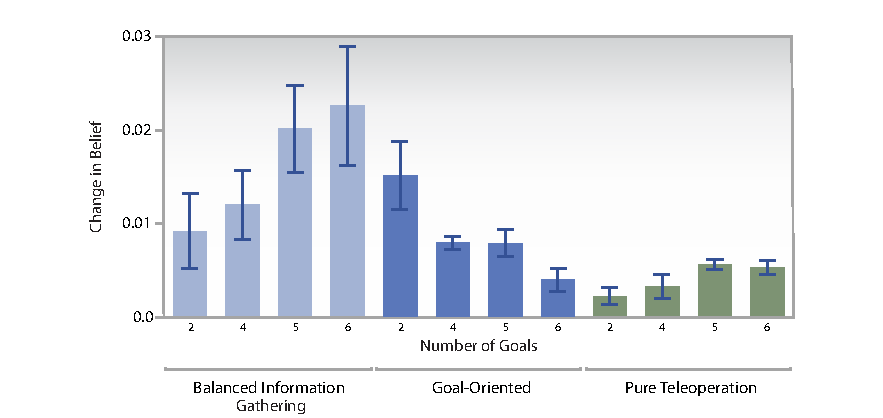
\includegraphics[width=\columnwidth]{figures/Info_Gain_By_Goal.pdf}
\caption{These plots demonstrate the differences in belief gain after shared autonomy windows separated by the number of candidate goals in the task.}
\label{goal_effect}
\end{figure}

\subsection{Limitations}

Our experimental data demonstrates mixed results on the use of active learning in teleoperation, with data suggesting that active learning may become more useful with more goals. However, our lack of significant findings on belief convergence speed show that further work is necessary to demonstrate scenarios in which such a system provides an advantage over purely goal-oriented systems.

\section{Conclusion}

Shared autonomy provides a means to augment human teleoperator's actions with those of a robotic system. Previous work has investigated ways to choose goal-oriented assistive actions, even without \textit{a priori} knowledge of user goals. We investigated the use of active information gathering actions within a shared autonomy paradigm in order to more quickly learn from the user's actions about their intended goal. We introduce a shared autonomy system for integrating information gathering actions and show trade-offs provided by information gathering compared to goal-oriented systems during user multitasking. Our data gives some insight into what kinds of scenarios may benefit from incorporating information gathering into shared autonomy, although further work is necessary to conclusively identify use cases with advantages for using such systems. Finally, the improvement that we found of both balanced information gathering and goal-oriented systems using hindsight optimization over pure teleoperation on belief convergence and task efficiency demonstrate the power of shared autonomy for a multitasking user.

\bibliographystyle{plainnat}
\bibliography{sample}

\end{document} 